\newcommand{\doctitle}{Numerical Methods Problem Sheet 1}
\providecommand{\doctitle}{Not Untitled}
\providecommand{\docauthor}{Nicolas Hafner}
\providecommand{\doccopyright}{Shirakumo}

\documentclass[12pt,a4paper,titlepage]{article}
\usepackage[utf8]{inputenc}
\usepackage[T1]{fontenc}
\usepackage[top=1.5cm, bottom=2.5cm, left=1cm, right=1cm]{geometry}
\usepackage{textcomp}
\usepackage{amsmath}
\usepackage{amsfonts}
\usepackage{amssymb}
\usepackage{amsthm}
\usepackage{fancyhdr}
\usepackage{fix-cm}
\usepackage{graphicx}
\usepackage{hyperref}
\usepackage{xcolor}
\usepackage{listings}
\usepackage{float}
\usepackage{wrapfig}
\usepackage{datetime}
\usepackage{enumitem}
\usepackage{minted}
\usepackage{epstopdf}

\newdateformat{dmny}{\monthname[\THEMONTH] \THEYEAR}
\newdateformat{dyo}{\THEYEAR}
\setlength{\headheight}{30pt}
\pagestyle{fancy}

\title{\doctitle}
\author{\docauthor}
\date{\d_mny\today}

\lhead{\docauthor}
\chead{\doctitle}
\lfoot{\copyright \dyo\today\; \doccopyright}
\cfoot{\thepage\ / \pageref{LastPage}}
\rhead{\dmny\today}

\definecolor{mintedbg}{rgb}{0.2,0.2,0.2}
\usemintedstyle{monokai}
\newmintedfile[matlabcode]{matlab}{
  bgcolor=mintedbg, fontfamily=tt,   linenos=true,     numberblanklines=true,
  numbersep=12pt,   numbersep=5pt,   gobble=0,         frame=leftline,
  framerule=0.4pt,  framesep=2mm,    funcnamehighlighting=true,
  tabsize=4,        obeytabs=false,  mathescape=false, samepage=false,
  showspaces=false, showtabs =false, texcl=false,
}

\newmintedfile[cppcode]{cpp}{
  bgcolor=mintedbg, fontfamily=tt,   linenos=true,     numberblanklines=true,
  numbersep=12pt,   numbersep=5pt,   gobble=0,         frame=leftline,
  framerule=0.4pt,  framesep=2mm,    funcnamehighlighting=true,
  tabsize=4,        obeytabs=false,  mathescape=false, samepage=false,
  showspaces=false, showtabs =false, texcl=false,
}

\renewcommand{\thesubsection}{\thesection.\alph{subsection}}


%%% Local Variables:
%%% mode: latex
%%% End:


\begin{document}
\begin{center}{\bfseries\Huge\doctitle}\end{center}

\section{Problem 1}
\subsection{}

$$ \left(\begin{array}{ccccc}
     d_1 & 0 & \hdots & 0 & a_1 \\
     0 & d_2 & \ddots & \vdots & a_2 \\
     \vdots & \ddots & \ddots & 0 & \vdots \\
     0 & \hdots & 0 & d_{n-1} & a_{n-1} \\
     a_1 & a_2 & \hdots & a_{n-1} & d_n
\end{array}\right) $$

\subsection{}

We are creating a Matrix $A$ of $n^2$ size. The matrix is then cubed, which is at worst an $O(n^3)$ operation. At smaller sizes constant overhead is going to dominate, explaining the divergence from $n^3$.

\subsection{}

\matlabcode{../arrowmatvec2.m}

\subsection{}

Since we just perform two Matrix multiplications with a vector we get a complexity of $O(n^2)$.

\subsection{}

\begin{figure}[h!]
  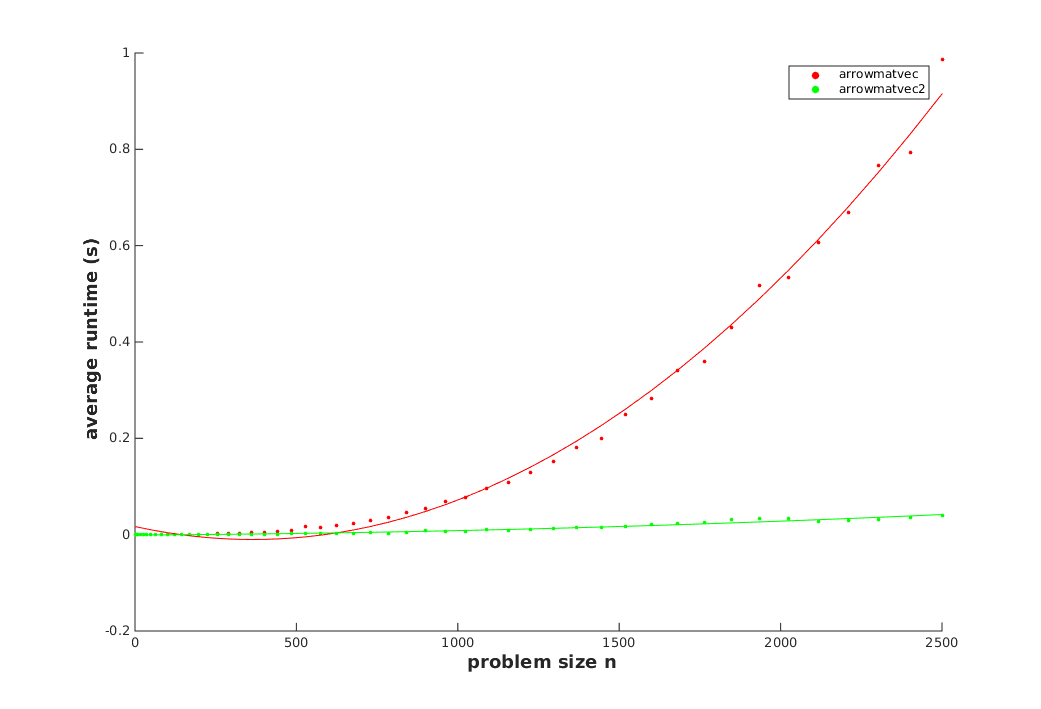
\includegraphics[scale=0.6]{./e1e.png}
\end{figure}

\subsection{}

\cppcode{../e1.cpp}

\end{document}

%%% Local Variables:
%%% mode: latex
%%% TeX-master: t
%%% TeX-engine: luatex
%%% TeX-command-extra-options: "-shell-escape"
%%% End:
